\documentclass{article}

% if you need to pass options to natbib, use, e.g.:
%     \PassOptionsToPackage{numbers, compress}{natbib}
% before loading neurips_2024
\PassOptionsToPackage{numbers, compress}{natbib}

% to compile a preprint version, e.g., for submission to arXiv, add add the
% [preprint] option:
%     \usepackage[preprint]{neurips_2024}


% to compile a camera-ready version, add the [final] option, e.g.:
%     \usepackage[final]{neurips_2024}


% to avoid loading the natbib package, add option nonatbib:
\usepackage[final]{neurips_2024}


\usepackage[utf8]{inputenc} % allow utf-8 input
\usepackage[T1]{fontenc}    % use 8-bit T1 fonts
\usepackage{hyperref}       % hyperlinks
\usepackage{url}            % simple URL typesetting
\usepackage{booktabs}       % professional-quality tables
\usepackage{amsfonts}       % blackboard math symbols
\usepackage{nicefrac}       % compact symbols for 1/2, etc.
\usepackage{microtype}      % microtypography
\usepackage{xcolor}         % colors
\usepackage{graphicx}       % graphics (added by Jeffery)
\usepackage{float}          % float (added by Jeffery)

% All packages added by Jeffery
\usepackage{graphicx} % Required for inserting images
\usepackage{tikz}
\usepackage{soul}
\usepackage{amsmath}
\usepackage{listings}
\usepackage{amssymb}
\usepackage{float}
\usepackage{parskip}
\usepackage{pgfplots}
\usepackage{xcolor}
\usepackage[shortlabels]{enumitem}
\usepackage{subcaption}

\newcommand*{\Perm}[2]{{}^{#1}\!P_{#2}}%
\newcommand*{\Comb}[2]{{}^{#1}C_{#2}}%
\newcommand*{\qed}{\hfill$\square$}%
\newcommand*{\txt}[1]{\text{ #1 }}%
\newcommand*{\iprod}[1]{\langle #1 \rangle}
\newcommand*{\fora}{\txt{}\forall}%
\newcommand*{\rr}{\mathbb{R}}%

\title{ UMD Building Classification }

\author{%
  Jerry Li\\
  \texttt{jli103@umd.edu} \\
  \And 
  Can Li \\
  \texttt{c5405@umd.edu} \\
  \And 
  Jeffery Tian \\
  \texttt{jtian12@umd.edu} \\
  \And 
  Christopher Lim \\
  \texttt{clim0326@umd.edu} \\
  \And 
  Justin Zhao \\
  \texttt{justinfz@umd.edu} \\
}


\begin{document}


\maketitle


%% TODO: 
%% Can's notes on data collection, FixMatch
%% https://arxiv.org/pdf/1412.6856
%% http://cnnlocalization.csail.mit.edu/Zhou_Learning_Deep_Features_CVPR_2016_paper.pdf
%% https://arxiv.org/pdf/1610.02391
%% https://github.com/kekmodel/FixMatch-pytorch
%% https://link.springer.com/article/10.1007/s10462-022-10246-w
%% 

\begin{abstract}
    With the rise of new computational architectures for image processing and classification, computer vision systems are highly diverse, raising the question of which approach is the most effective for a given task. Our study focuses on designing and evaluating a reliable classification system for identifying buildings on the University of Maryland campus using semi-supervised CNN. By constructing a custom image database from scratch and experimenting with various architectures for semi-supervised learning, we aim to identify the best model for our classification problem. Additionally, we utilize CNN visualization eg. Grad-CAM to further assess our model’s performance.
\end{abstract}


\section{Motivation}
\label{motivation}

Although not addressing an urgent problem, our goal was to gain experience with the entire deep learning lifecycle, from data acquisition to final model evaluation. We built our own image database from scratch and conducted extensive experiments with a variety of supervised and semi-supervised learning models to ensure the highest accuracy.

The challenge came from the fact that we had to build our own dataset from scratch. We additionally worked with implementation of high resolution images on limited datasets to semi-supervised methods, along with the use of Grad-CAM for image segmentation.

We additionally did experiments on GNNs and HITL with Grad-CAM.

\subsection{Related Works}

Much work has been done with relation to image segmentation of multiple relevant objects (eg. buildings) and their classification.

\begin{itemize}
    \item On the topic of image recognition/classification, AlexNet, VGG, and Resnet\cite{krizhevsky}\cite{simonyan}\cite{he} are strong examples of fully supervised traditional CNN recognition and classification models. 
    \item With respect to image segmentation, we end up using Grad-CAM as detailed after this section.
\end{itemize}

This also includes significant work being done on visual explanations of CNN models via Selvaraju, et al.\cite{selvaraju} (2019) Grad-CAM and other related works. These can be used as an alternative method of segmentation and recognition. Below we discuss the main works of relevance to our work:

We prioritized utilizing Semi-Supervised Methods of image recognition. For this, we used FixMatch and MeanTeach methods. 

\begin{itemize}
    \item FixMatch, Sohn, et al.\cite{sohn} (2020), is a semi-supervised learning method that generates “pseudo-labels” using model predictions on weakly augmented unlabeled data, retained only if it’s high confidence; then, train to predict that pseudo label with a strongly augmented version.

    This is a strong method for semi-supervised learning with limited datasets, so will be one of our main driving methods of implementation.
    \item MeanTeacher, Tarvainen, et al.\cite{tarvainen} (2017), is a semi-supervised learning method that uses a teacher model to provide a consistent target for the student model. The teacher model is an exponential moving average of the student model, and the student model is trained to match the teacher model’s predictions.
\end{itemize}

% Write: how gradcam can help find the location of the building in the image (to help find its not on the foreground images), point out how this isn't the case in prelim

\begin{itemize} % IP: Gradcam, Scorecam, Gradcam++
    \item Grad-CAM, Selvaraju, et al.\cite{selvaraju} (2019), uses the final gradient into the last convolution layer to produce a visual representation of strength in decision making. This is a visual indicator of model strength and is on paper highly useful for highlighting image classification confidence, but can also be used to help define segmentation. 
    % https://arxiv.org/abs/1610.02391 gradcam
    \item Grad-CAM++, Chattopadhay, et al.\cite{chattopadhay} (2018) is an upgrade to Grad-CAM by generalizing it. It can then isolate/identify multiple object instances in a single image (important for our proposal due to the presence of multiple buildings in images) and a generally improved visual indicator. 
    % https://arxiv.org/abs/1710.11063 gradcam++
\end{itemize}

Grad-CAM++ can be used as an important means for highlighting image classification confidence, both of which we intend to use as the most advanced methods in their respective lineages. As an example, see our Grad-CAM results in Appendix \ref{extra_figures} on instances on our test set. This can be used for confirmation of model confidence. If the model is sufficiently confident, this can even be used as a means to indicate building locations (especially given Grad-CAM++ ability to find multiple instances) within the image rather than using traditional segmentation techniques.

We additionally used GNN methods and HITL methods. \begin{itemize}
    \item Graph Neural Networks are a method of using graph data to make predictions. This can be used to make predictions on the labeled/unlabeled samples as nodes, and should this perform reasonably this can be used as a primary paradigm as well. 
    
    The main motivator for this is that nodes can be connected by edges to represent relationships that go beyond stride.

    Long et al.\cite{long} (2020) is prior work on GNN image recognition, done on the MNIST dataset on low resolution black and white images. Our intention is to innovate by extending this to high resolution color images of buildings.

    \item Superpixels are a method of dividing an image into regions of similar color. This can be used to help segment the image and can be used to help the model focus on the building itself. This is a method of image segmentation that can be used to help the model focus on the building itself. For graphs, this is a method of reducing the complexity greatly. 

    The SLIC-Superpixel transform, developed by EPFL labs \cite{epflSLICSuperpixels}, is a method of superpixel generation that can be used to help segment the image. This can be used to focus node complexity on details.
    \item HITL is human corrections on the network to help the network focus on areas of interest by providing absolute feedback on whether or not Grad-CAM is focusing on the correct areas.
\end{itemize}

\subsection{Motivation for Methods}

From these prior works we have the basic motivation of leveraging traditional CNN image segmentation and recognition techniques for the sake of identifying any buildings in the input images. Our main innovation is to attempt to use Grad-CAM++ or a similar technique to see if they can be used for image segmentation instead, and to attempt to apply this basic system to a variety of goals.

The focus is to see if we can get Grad-CAM to focus on the elements of the image that are important, to help "guide" the model to focus on the building itself. This is important because the model may be making predictions based on unrelated objects in the image, and this can be used to confirm model confidence.

\section{Methods}
\label{method}

\subsection{Data Collection}

Data was collected by individually taking pictures and labeling them, along with data augmentation. We took around 4000 photos of UMD buildings over 20 classes, aiming for a 60/40 split of daytime/nighttime photos. Buildings included a diverse set of buildings but also included 4 dorms of extremely similar construction.

Care was taken to ensure that the photos were taken from a variety of angles and distances. We were limited in time and season since data collection occurred mainly over the course of 2 weeks in fall. 

%% TODO: insert figure.

The dataset was split 80/10/10 for training/validation/testing. Photos were augmented by displacement and inherently varied by rotation. All images were resized to 224x224 for training. 

Test images were further augmented by adding noise and other transforms, including the SyRA synthesized rain (Choi et al. \cite{choi}) method to add rain streaks to the images. 

Further augmentation methods were done for training via contrast, brightness, colorspace, cutout, rotation, sharpness, shearx, inversion, solarization, and translation methods. For FixMatch, we followed a standard augmentation pipeline of the above; details can be seen in our github.

\subsection{Fully Supervised Baseline}

A fully supervised model was implemented using various ResNet/VGG models for the sake of both comparison and as a baseline for our semi-supervised methods. After training ResNet18 was determined to be best with a 97.63\% validation accuracy on test set after only 12 epochs. 

We achieved this using the pretrained ResNet18 model and fine-tuning it over our dataset. Code and parameters can be found in the Github repository. The primary function of the FS model was to provide a baseline for our semi-supervised methods.

\subsection{Semi-Supervised Methods}

We utilized 2 methods of semi-supervised learning: FixMatch and MeanTeacher. Both were supplemented by Grad-CAM

\subsubsection{Grad-CAM}

Grad-CAM visualizes the last layer of the CNN structure with heatmaps, and is a generalization of the CAM method. In the Grad-CAM process, a forward pass is done to compute the class score for target class $c$. Then, gradients are backpropagated on the target class score $y^c$ (before softmax), wrt. the feature maps of each convolutional layer, $A^k$. That is, $\forall k \in \{1, 2, ..., K\}$, we compute the gradient of $\frac{\partial y^c}{A^k}$. Then, the importance of the weight $a_k^c\in A^k$ is computed as \begin{align*}
    a_k^c=\frac{1}{Z}\sum_i\sum_j\frac{\partial y^c}{A_{ij}^k}
\end{align*} where $Z$ is the total number of spacial locations in the feature map. Then, the final feature map is calculated as \begin{align*}
    \mathcal{L}_{Grad-CAM}^c=\text{ReLU}\left(\sum_k a_k^cA^k\right)
\end{align*}

While Grad-CAM can show us the heatmap, the Grad-CAM paper by Selvaraju et al. \cite{selvaraju} notes that it lacks the ability to show us the fine grained details like pixel-space gradient visualization, such as Guided Backpropagation. 


\begin{figure}[H]
    \centering
    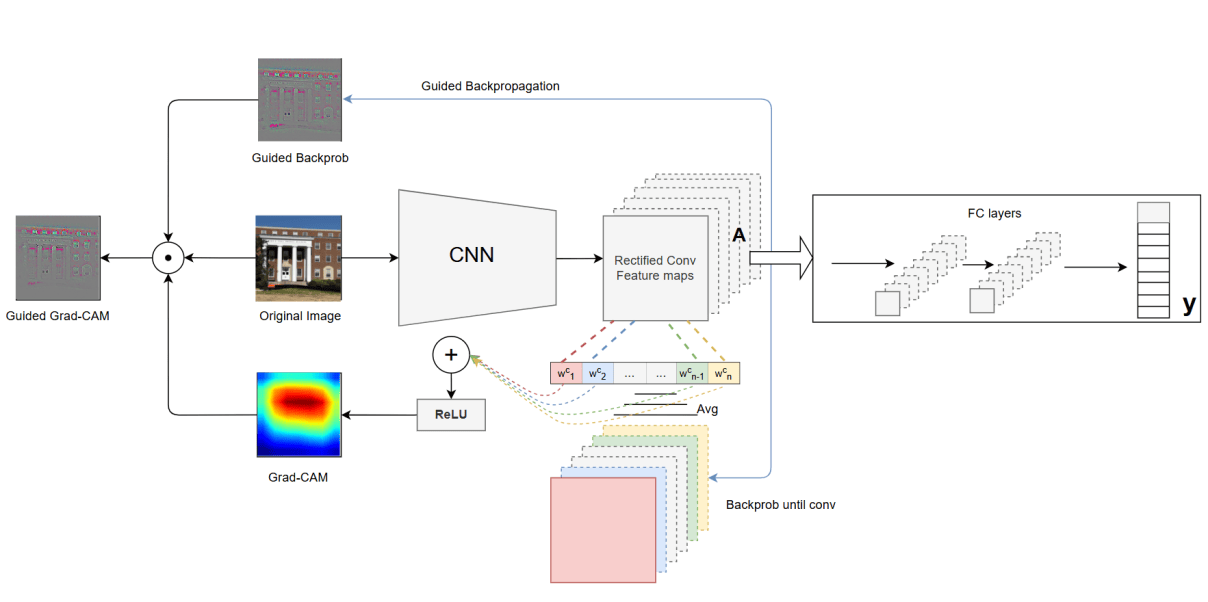
\includegraphics[width=0.8\linewidth]{model_architecture.png}
    \caption{Grad-CAM Model Architecture}
    \label{fig:gradcam_architecture}
\end{figure}

Guided Backpropagation is a variant of the backpropagation algorithm where negative gradients are suppressed during the backward pass. Only positive gradients are propagated, highlighting the pixels in the input image that strongly activate certain neurons in the network. This will result in a high-resolution saliency map of the input image. To combine it with Grad-CAM, we can multiply the Grad-CAM heatmap with the Guided Backpropagation saliency map element-wise to get the Guided Grad-CAM result.  

\begin{figure}[H]
    \centering
    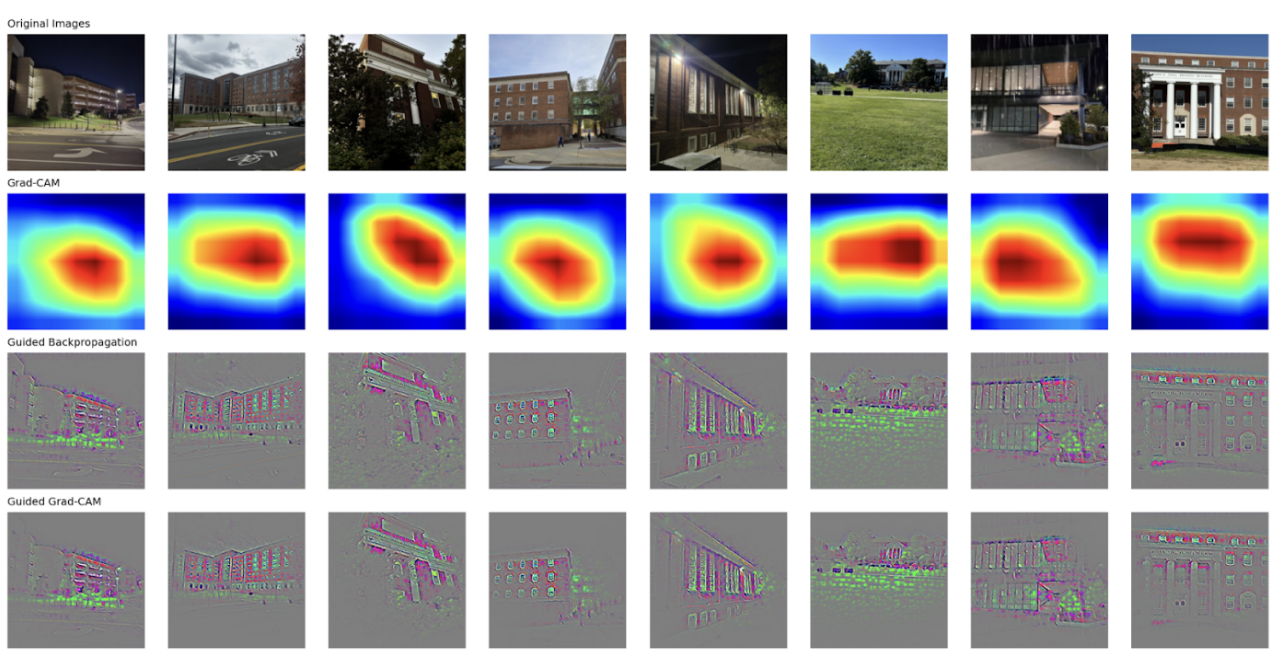
\includegraphics[width=0.8\linewidth]{gradcam_demo.png}
    \caption{Grad-CAM visualization demo}
    \label{fig:gradcam_demo}
\end{figure}
%% TODO: insert figure.
Grad-CAM++ works by assigning importance weights to individual pixels in the feature maps, rather than the global pooled gradients used in Grad-CAM, allowing it to better capture fine-grained details and spatial information. This pixel-level weighting enables Grad-CAM++ to provide more localized and precise visual explanations, especially in cases where multiple instances of the same class are present in an image. Despite this theoretical improvement, the results we obtained did not show significant differences compared to Grad-CAM, potentially due to limitations in model architecture, dataset complexity, or specific implementation nuances.

\subsubsection{FixMatch}

Our FixMatch model generated pseudo-labels for unlabeled data using weakly augmented data (eg. rotation, translation, etc.) and trained to predict these pseudo-labels with strongly augmented data (eg. cutout, solarization, color space, etc.).

We trained a variety of different models with different hyperparameters (batch size, momentum, warm up epochs, pseudo label threshold, etc) and selected 5 for further testing. Parameters can be found on the github in \verb*|CMSC472_Final_Project/code/my_fixmatch/dataset/parms.ipynb|. All images were standardized at 224x224, using the SyRA synthesized rain test image set with a random augmentation pipeline. 

Models 1, 2 were trained for 128 epochs, and 3, 4, 5 for 32 over the WideResNet model with depth 16, widen factor 2, and dropout 1. Each model was trained on the previous, iteratively. The model was trained on the 20 classes of UMD buildings, on a NVIDIA RTX 3090. All code is available on the Github repository.

\subsubsection{MeanTeacher}

Our MeanTeacher model uses consistency regularization that requires 2 models: a student model and a teacher model. The teacher model is an exponential moving average of the student model, and the student model is trained to match the teacher model’s predictions.

Our student network acts as the standard neural network, trained on both supervised and unsupervised losses. Our teacher network acts as the target for the student. 

For labeled data, the student network is trained to minimize supervised loss via cross-entropy. For unlabeled data, the student network is trained to minimize the consistency loss between the student and teacher predictions.

All data went to both of our models, where it was then augmented with random horizontal translations and translations (eg. weak augmentation). We utilized MSE loss for consistency loss in unlabeled data. For labeled data, we utilized the weights formula \begin{align*}
    \theta_{\text{teacher}}=\alpha \cdot\theta_{\text{teacher}}+(1-\alpha)\cdot\theta_{\text{student}}
\end{align*} where $\alpha$ is the decay rate. Final loss was calculated as \begin{align*}
    \mathcal{L}_{\text{total}}=\mathcal{L}_{\text{supervised}}+\lambda\cdot\mathcal{L}_{\text{consistency}}
\end{align*}where $\lambda$ was the weight of the consistency loss.

The model was trained for 25 epochs over the ResNet18 model. The model was trained on the 20 classes of UMD buildings, on Google Colab with a Tesla T4 GPU. All code is available on the Github repository.

\subsection{GNNs/HITL Experiments}

We additionally experimented with GNNs (Graph Neural Networks), HITL (Human In The Loop), and VQA (Visual Question Answering) methods. Results for these can be found in appendix \ref{experiment_results}.

VQA was found to be infeasible due to time constraints; the amount of questions required was too high given our priorities on semi-supervised learning and the lack of time we allotted to the experiment.
% results for these will go into appendix

\subsubsection{HITL}

HITL, or Human In The Loop, is a method to accelerate the training of a model by providing human feedback on the model's predictions. This can be used to help the model focus on areas of interest by providing absolute feedback on whether or not Grad-CAM is focusing on the correct areas.

We implemented a model on 9 classes and a train set of 450 images, where humans were asked to provide feedback on the accuracy of class predictions and whether or not the Grad-CAM feedback was accurate (eg. not focusing on noise). The model was implemented for PyTorch and was trained on Colab with a Tesla T4 GPU for 10 epochs, with human interference once per epoch. 

After each epoch, the human was asked to confirm or deny the accuracy of the model's prediction, and asked a region of the image for the model to focus on more based on the Grad-CAM feedback.

A ResNet18 model was used, with 10 epochs, $lr=0.001$, batch size 64. 

\subsubsection{GNNs}

Images for GNNs were standardized to 224x224, then ran through our custom implementation of the SLIC Superpixel transform to \verb*|torch_geometric(Data)| objects. Edges were generated via a Radius Neighbor Graph with varying parameters. The transform method is adapted from low resolution B/W to high resolution color images at variable resolution.

To visualize the model and SLIC transform, methods were written to represent the graph in 2d space.

Our GNN classifier was implemented in PyTorch Geometric, following the method outlined in Long et al \cite{long}. The method uses a 3 layer GatConv model with a FC layer at the end. The model was initially trained on fully supervised data, but could not complete due to time constraints. Training was done on the Columbia \@ SAIL server with an NVIDIA RTX A6000 GPU. It is intended to train on 100 epochs, and a hidden dimension of 152. 

The SLIC transform results in significant preprocessing costs, and was the main cost of the model. All code is available on the Github repository, although no results are provided.

\section{Experiment Results}
\label{result}
% Demonstrate stats

\subsection{Fully Supervised Baseline}

We trained various ResNet/VGG models for the fully supervised baseline. After training, ResNet18 was determined to be the best model for semisupervised with a 97.63\% validation accuracy on the test set after 12 epochs. All training was done on the 20 classes of UMD buildings, on Google Colab with a Tesla T4 GPU. All code is available on the Github repository.

All testing was done on the heavily augmented test set to check for robustness, and we achieved the following peak accuracies for the models within 25 epochs:

\begin{table}[H]
    \centering
    \begin{tabular}{|c|c|c|}
        \hline
        Architecture & Best Val Accuracy & Test Accuracy \\
        \hline
        DenseNet121 & 98.26\% & 87.77\% \\
        \hline
        DenseNet201 & 97.00\% & 87.93\% \\
        \hline
        ResNet18 & 97.63\% & 88.54\% \\
        \hline
        ResNet34 & 98.89\% & 86.38\% \\
        \hline
        ResNet50 & 96.05\% & 80.13\% \\
        \hline
    \end{tabular}
    \caption{Comparison of DenseNet/ResNet Model Accuracies}
    \label{tab:dnrn_model_accuracies}
\end{table}

The following VGG/VIT models were also tested, but were found to be less effective than the ResNet models.

\begin{table}[H]
    \centering
    \begin{tabular}{|c|c|c|}
        \hline
        Architecture & Val Accuracy & Test Accuracy \\
        \hline
        VGG11 & 84.36\% & 55.73\% \\
        \hline
        VGG16 & 79.94\% & 78.84\% \\
        \hline
        VGG19 & 80.09\% & 41.33\% \\
        \hline
        Vit16\_224 & 69.04\% & 42.62\% \\
        \hline
    \end{tabular}
    \caption{Comparison of VGG/VIT Model Accuracies}
    \label{tab:vgg_model_accuracies}
\end{table}
\subsection{Semi-Supervised Methods}
\subsubsection{FixMatch}

Our FixMatch method achieved peak top1 accuracy of 40.45\% and top5 accuracy of 75.44\%, where top1 indicates a correct guess within the most confident prediction and top5 indicating a correct guess on the top 5 most confident predictions.

\begin{table}[H]
    \centering
    \begin{tabular}{|c|c|c|}
        \hline
        Model & Top-1 Accuracy & Top-5 Accuracy \\
        \hline
        1 & 27.95\% & 61.25\% \\
        \hline
        2 & 30.44\% & 64.50\% \\
        \hline
        3 & 38.75\% & 75.08\% \\
        \hline
        4 & 40.45\% & 75.44\% \\
        \hline
        5 & 19.20\% & 68.37\% \\
        \hline
    \end{tabular}
    \caption{Comparison of Model Accuracies}
    \label{tab:fm_model_accuracies}
\end{table}

The FixMatch model fell into the issue of overfitting on our dataset fairly quickly due to the relatively small per-class dataset. This was exacerbated by the limited weather conditions and time of day we took photos, which resulted in a lack of diversity and strong overfitting on nonexistent features. 

However, we were successful in locking Grad-CAM onto building features, and we achieved reasonable test accuracies on the heavily augmented SyRA test set. If time permits, we would like to add more labeled data to the dataset and see if the result improves. 

\begin{figure}[H]
    \centering
    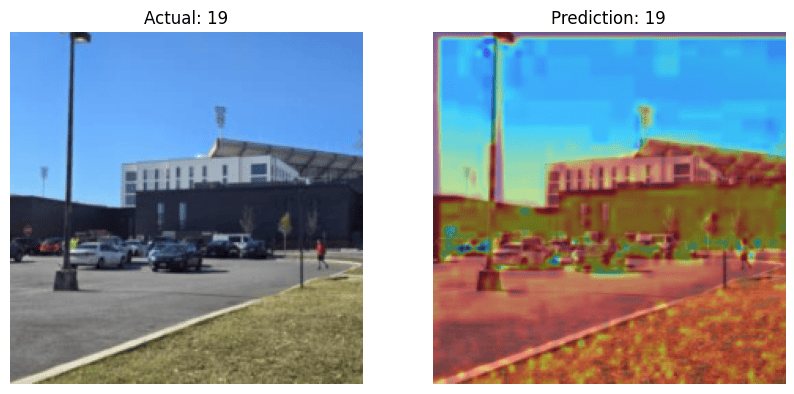
\includegraphics[width=0.8\linewidth]{fixmatch.png}
    \caption{FixMatch Model Grad-CAM visualization}
    \label{fig:fixmatch_results}
\end{figure}

\subsubsection{MeanTeacher}

Our MeanTeacher model achieved top1 student accuracy of 75.08\% and top1 teacher accuracy of 73.89\%. This utilized $\lambda=1.5, \alpha=.99$, with $lr=0.001$, batch size $128$, SGD decay $10^{-4}$, and momentum $.9$ over 20 epochs.

The MeanTeacher model performed significantly better than the FixMatch model due to its consistency regularization. The model was able to generalize better to the test set and was less prone to overfitting. 

However, it still suffered from the same lack of diversity. Once again, we were successful in locking Grad-CAM onto building features, and we achieved reasonable test accuracies on the heavily augmented SyRA test set.

\begin{figure}[H]
    \centering
    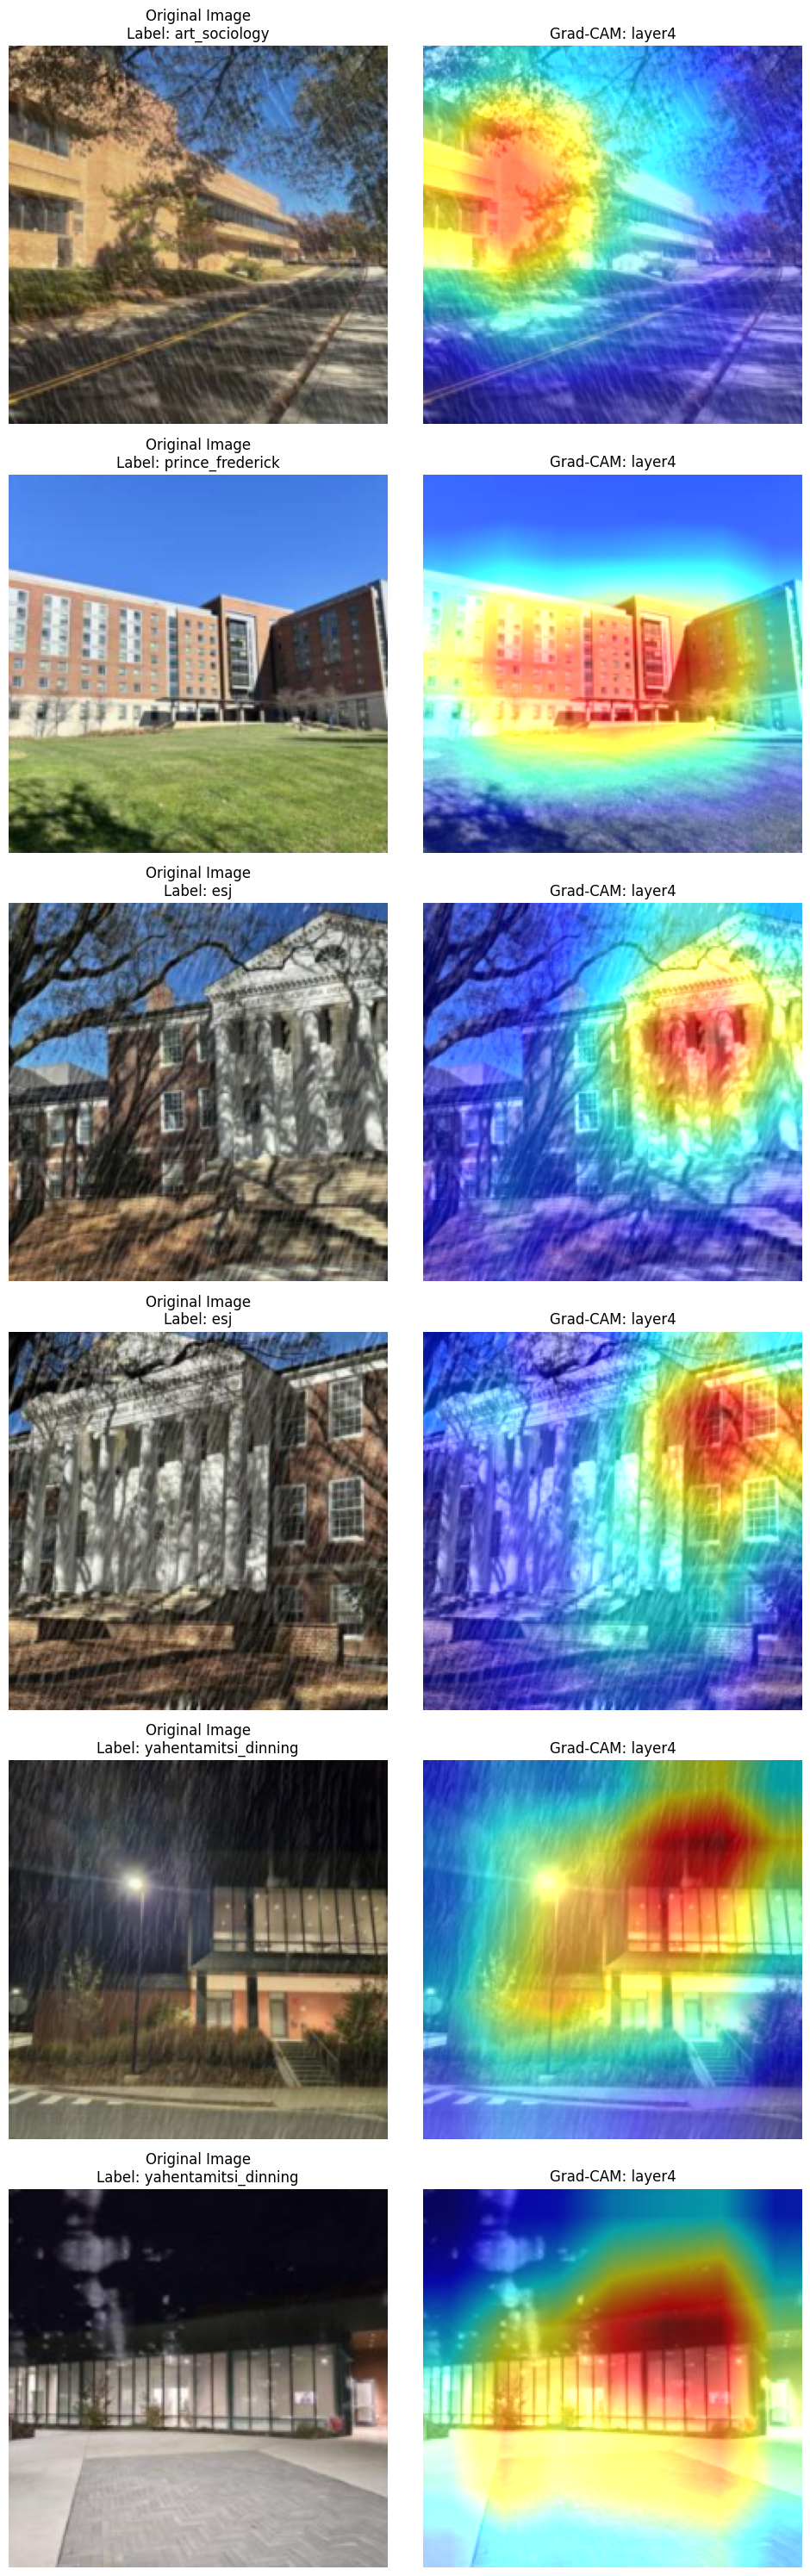
\includegraphics[trim={0 38cm 0 12.5cm},clip,width=0.6\linewidth]{meanteacher.png}
    \caption{MeanTeacher Model Grad-CAM visualization}
    \label{fig:meanteacher_results}
\end{figure}
% Demonstrate stats

\section{Conclusion}

Our key findings are that for the classification of buildings, ResNet18 is the best baseline model; and that MeanTeacher outperformed FixMatch considerably, achieving a top1 student accuracy of 75.08\% and top1 teacher accuracy of 73.89\%. Extensive quantitative findings prove that it's also much more robust to overfitting than FixMatch, and reacts better to an augmented test set. For both, we were successful in locking Grad-CAM onto building features. 

However, both models suffered from a lack of diversity in the dataset, which led to overfitting on nonexistent features and a lack of improvement. Advancement on FixMatch can be achieved via cleaning up the dataset (eg less noise). Additionally, multiple classes can be defined for various parts of buildings (i.e. Atlantic Building looks very different depending on the angle).

For our dataset, after trying various network architectures, we learned that having deep layers won’t simply improve the prediction accuracy (and can easily result in overfitting). In the ResNet family, for example, ResNet50 performed less accurately compared to ResNet18. Another interesting result we got is that in the VGG family, the test data showed us that VGG16 > VGG11 > VGG19 accuracy-wise. Thus, networks with not enough layers can also cause a difference.  

Future research will focus on increasing the diversity of the dataset, along with continuing preliminary work on GNNs. We would also like to experiment with more fine tuning of parameters and warm up functions.

\subsection*{GitHub Repository}

All code and resources for this project are available at: \url{https://github.com/BlueTurtle123/CMSC472_Final_Project}

\newpage 
\appendix

\section{Extra Experiment Results}
\label{experiment_results}

\subsection{HITL}

After 10 epochs, the model achieved training accuracy $93.74\%$, and test accuracy $67.6\%$. 

\begin{figure}[H]
    \centering
    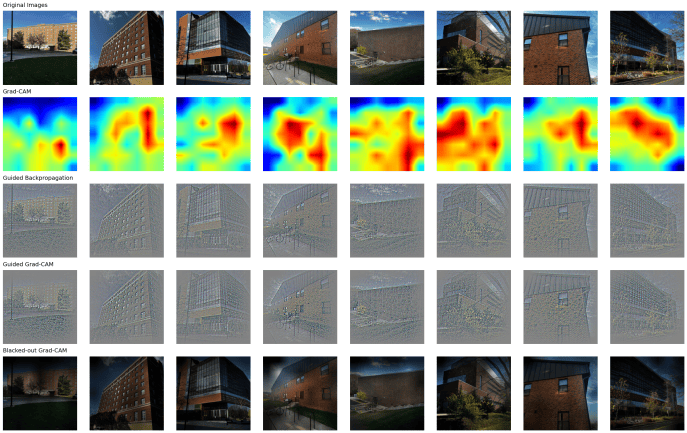
\includegraphics[width=0.8\linewidth]{hitl.png}
    \caption{HITL Model Grad-CAM visualization}
    \label{fig:hitl_results}
\end{figure}

\subsection{GNNs}

The GNN model was unable to complete training due to time constraints. However, we did complete our SLIC transform, for which we have the following figures:

\begin{figure}[H]
    \centering
    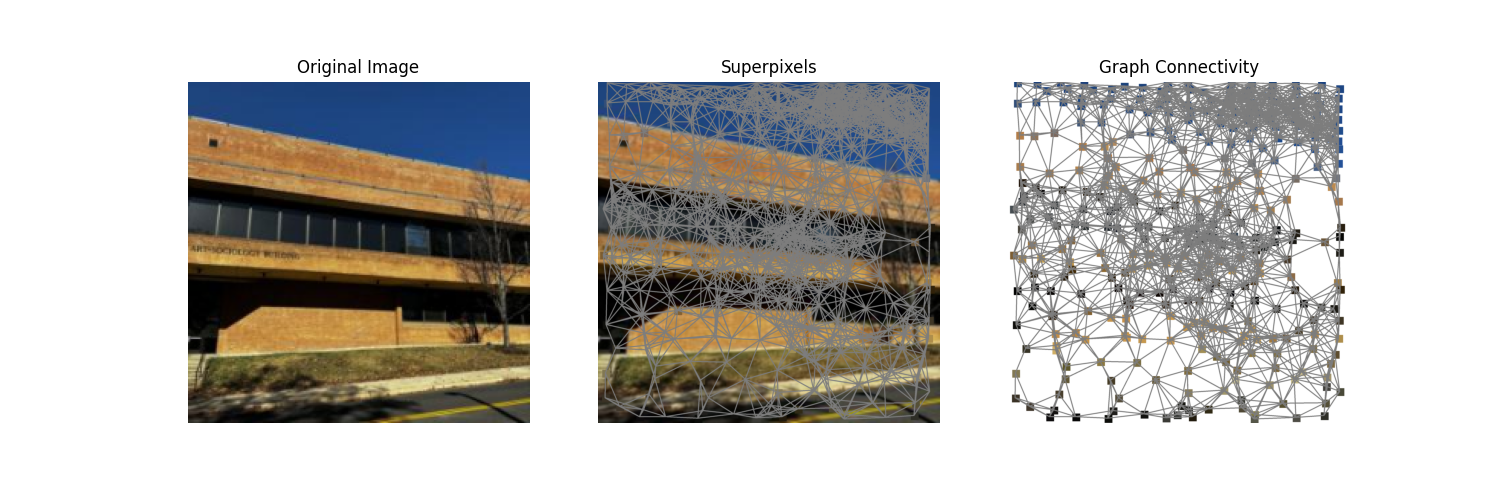
\includegraphics[width=0.8\linewidth]{slic_1.png}
    \caption{SLIC transform of Art-Sociology building picture}
    \label{fig:slic1}
\end{figure}

\begin{figure}[H]
    \centering
    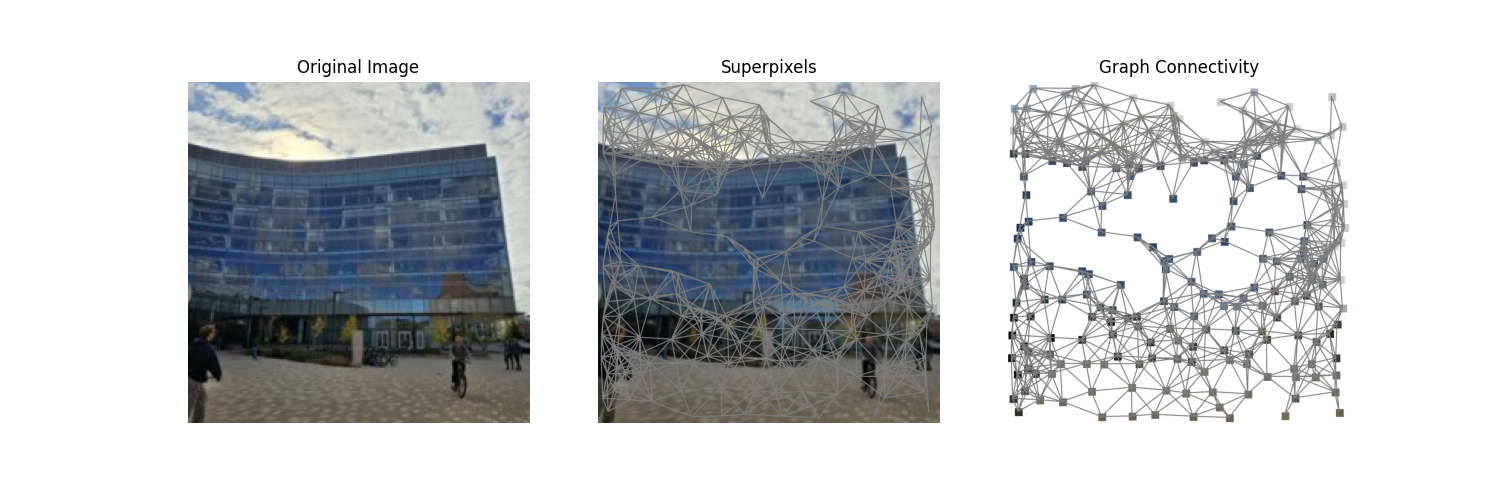
\includegraphics[width=0.8\linewidth]{slic_2.png}
    \caption{SLIC transform of Iribe building picture}
    \label{fig:slic2}
\end{figure}

Note how in the pictures, excessive complexity is granted to largely irrelevant details, such as the clouds and sky. Minute differences in the image data due to noise result in a lack of clustering in those areas. 

\section{Extra Figures}
\label{extra_figures}

\begin{figure}[H]
    \centering
    % First subfigure
    \begin{subfigure}[b]{0.45\linewidth}
        \centering
        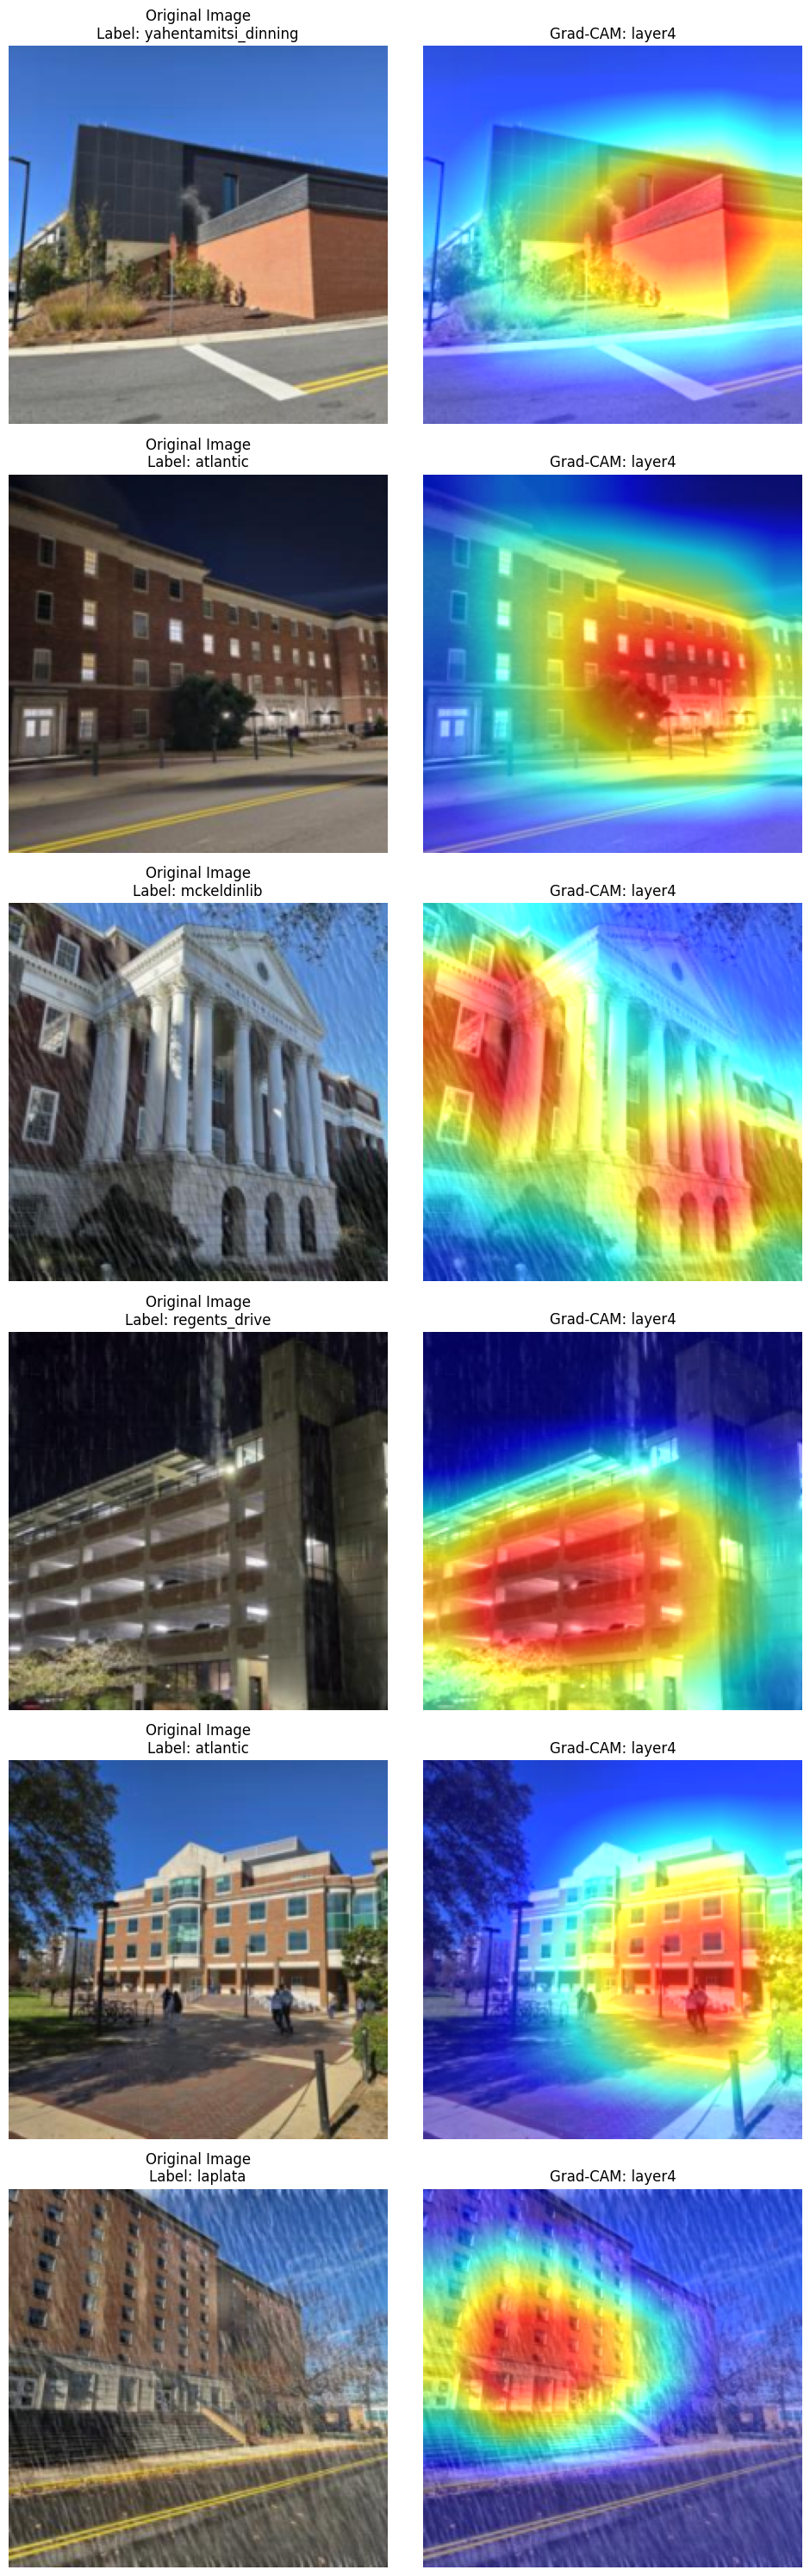
\includegraphics[width=\linewidth]{new_gradcam_result2.png}
        \caption{Grad-CAM visualization on ResNet18}
        \label{fig:gradcam1}
    \end{subfigure}
    \hfill  % Adds horizontal spacing
    % Second subfigure
    \begin{subfigure}[b]{0.45\linewidth}
        \centering
        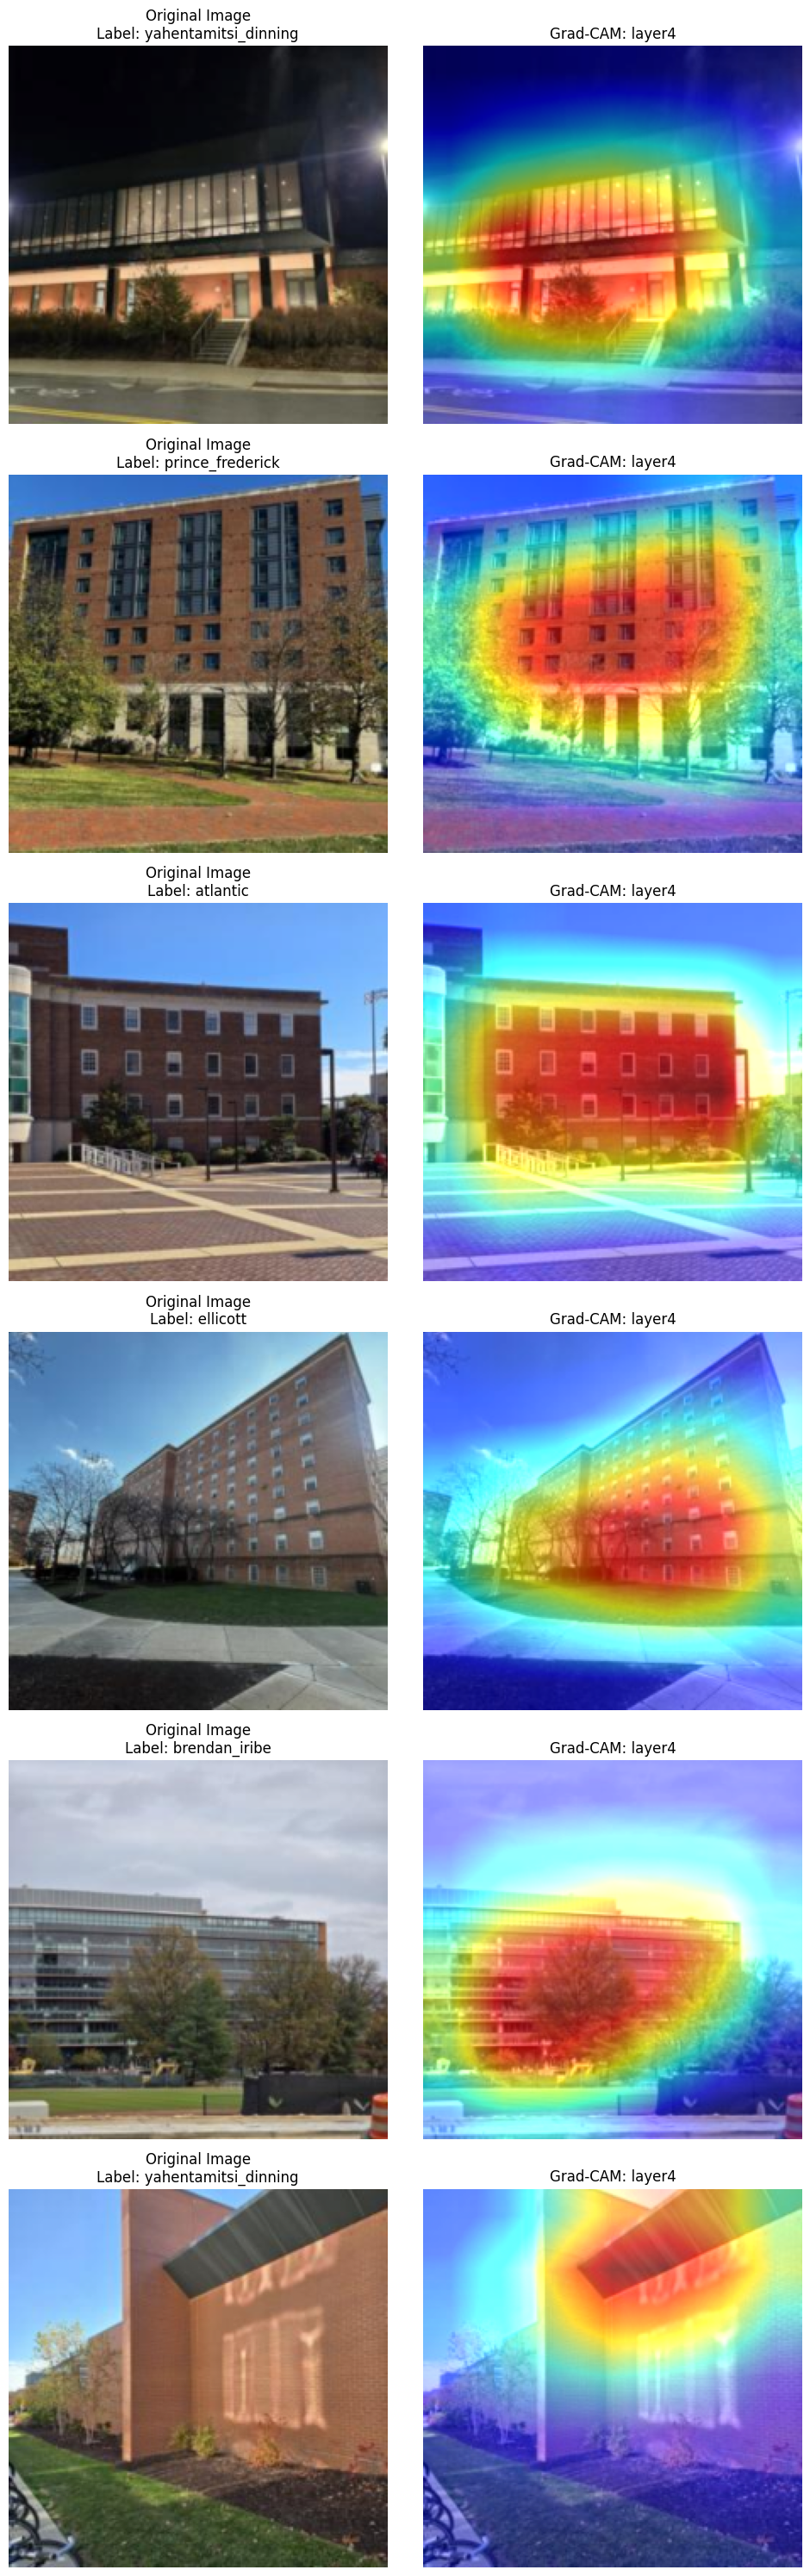
\includegraphics[width=\linewidth]{new_gradcam_plusplus_result2.png}
        \caption{Grad-CAM++ visualization on ResNet18}
        \label{fig:gradcam2}
    \end{subfigure}

    \caption{Comparison of Grad-CAM and Grad-CAM++ visualizations on ResNet18}
    \label{fig:gradcam_comparison1}
\end{figure}

\begin{figure}[H]
    \centering
    % First subfigure
    \begin{subfigure}[b]{0.45\linewidth}
        \centering
        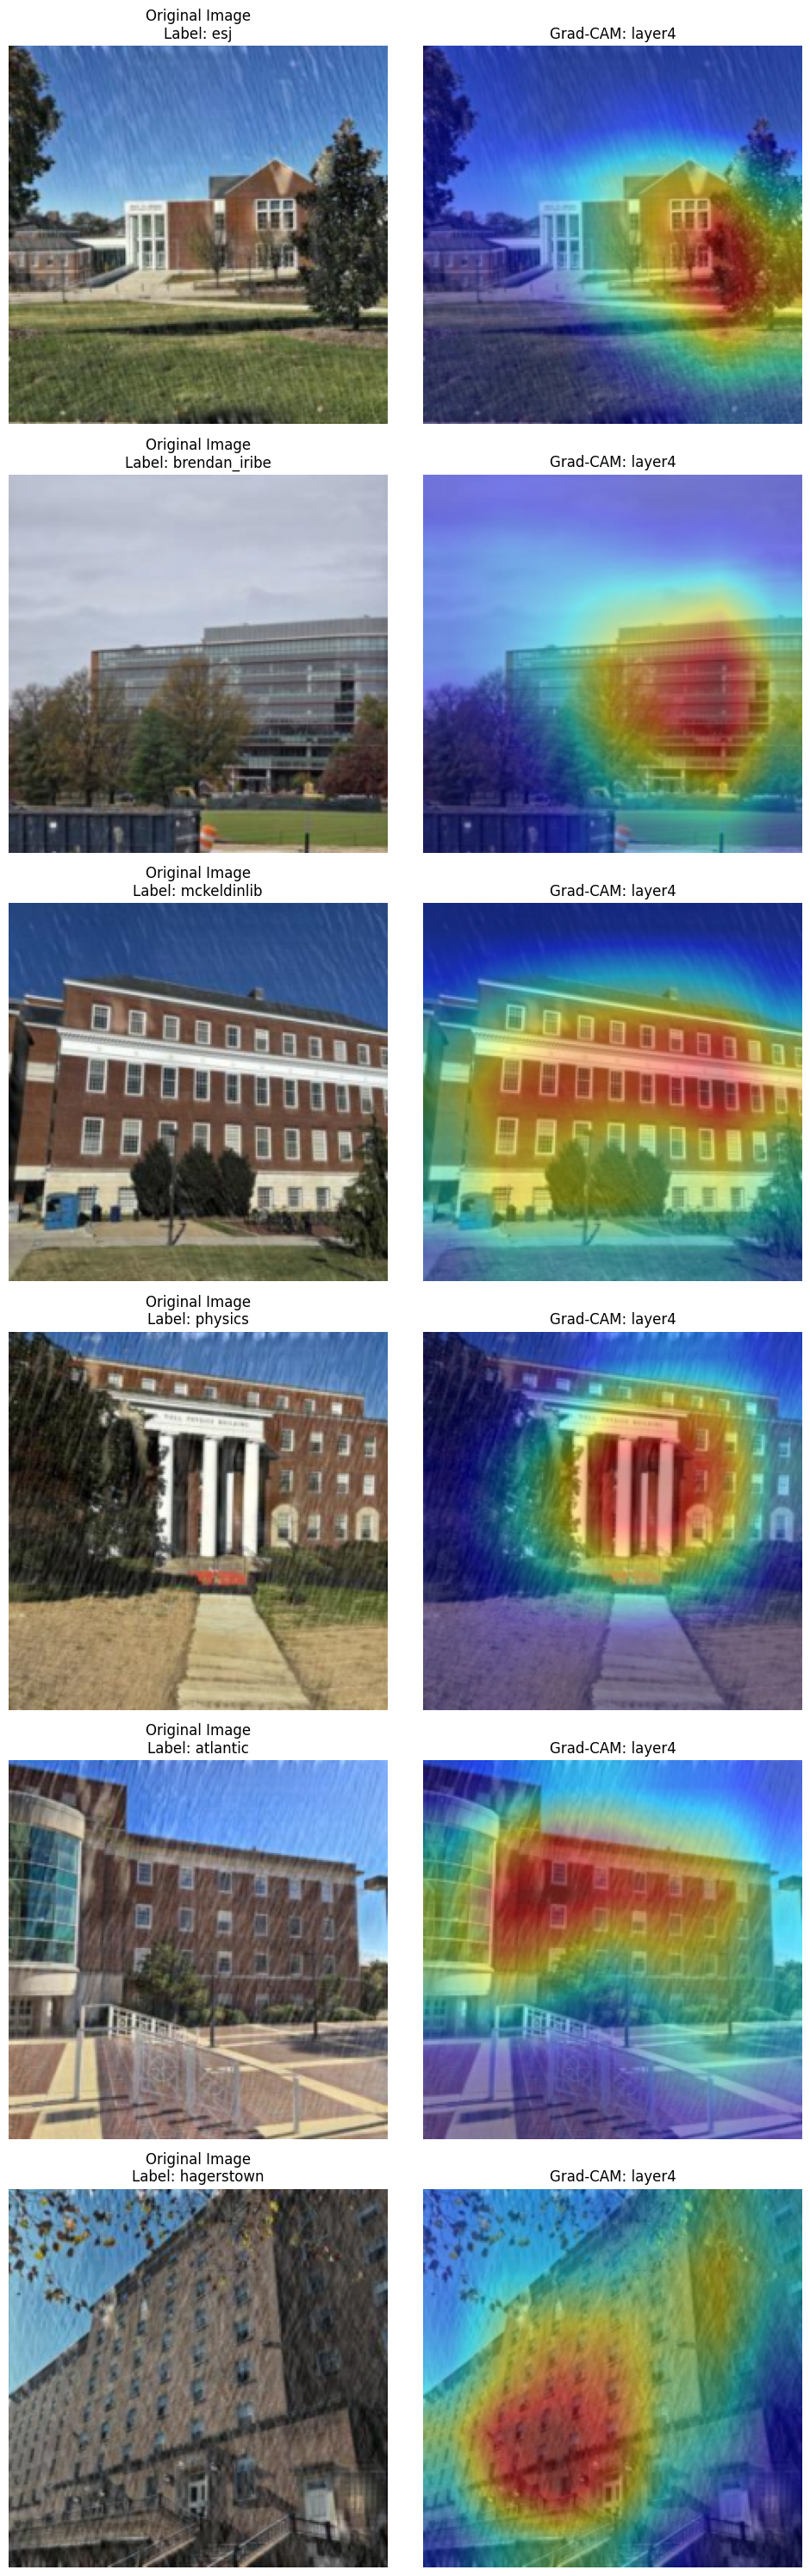
\includegraphics[width=\linewidth]{gradcam_result3.png}
        \caption{Grad-CAM visualization on MeanTeach}
        \label{fig:gradcam3}
    \end{subfigure}
    \hfill  % Adds horizontal spacing
    % Second subfigure
    \begin{subfigure}[b]{0.45\linewidth}
        \centering
        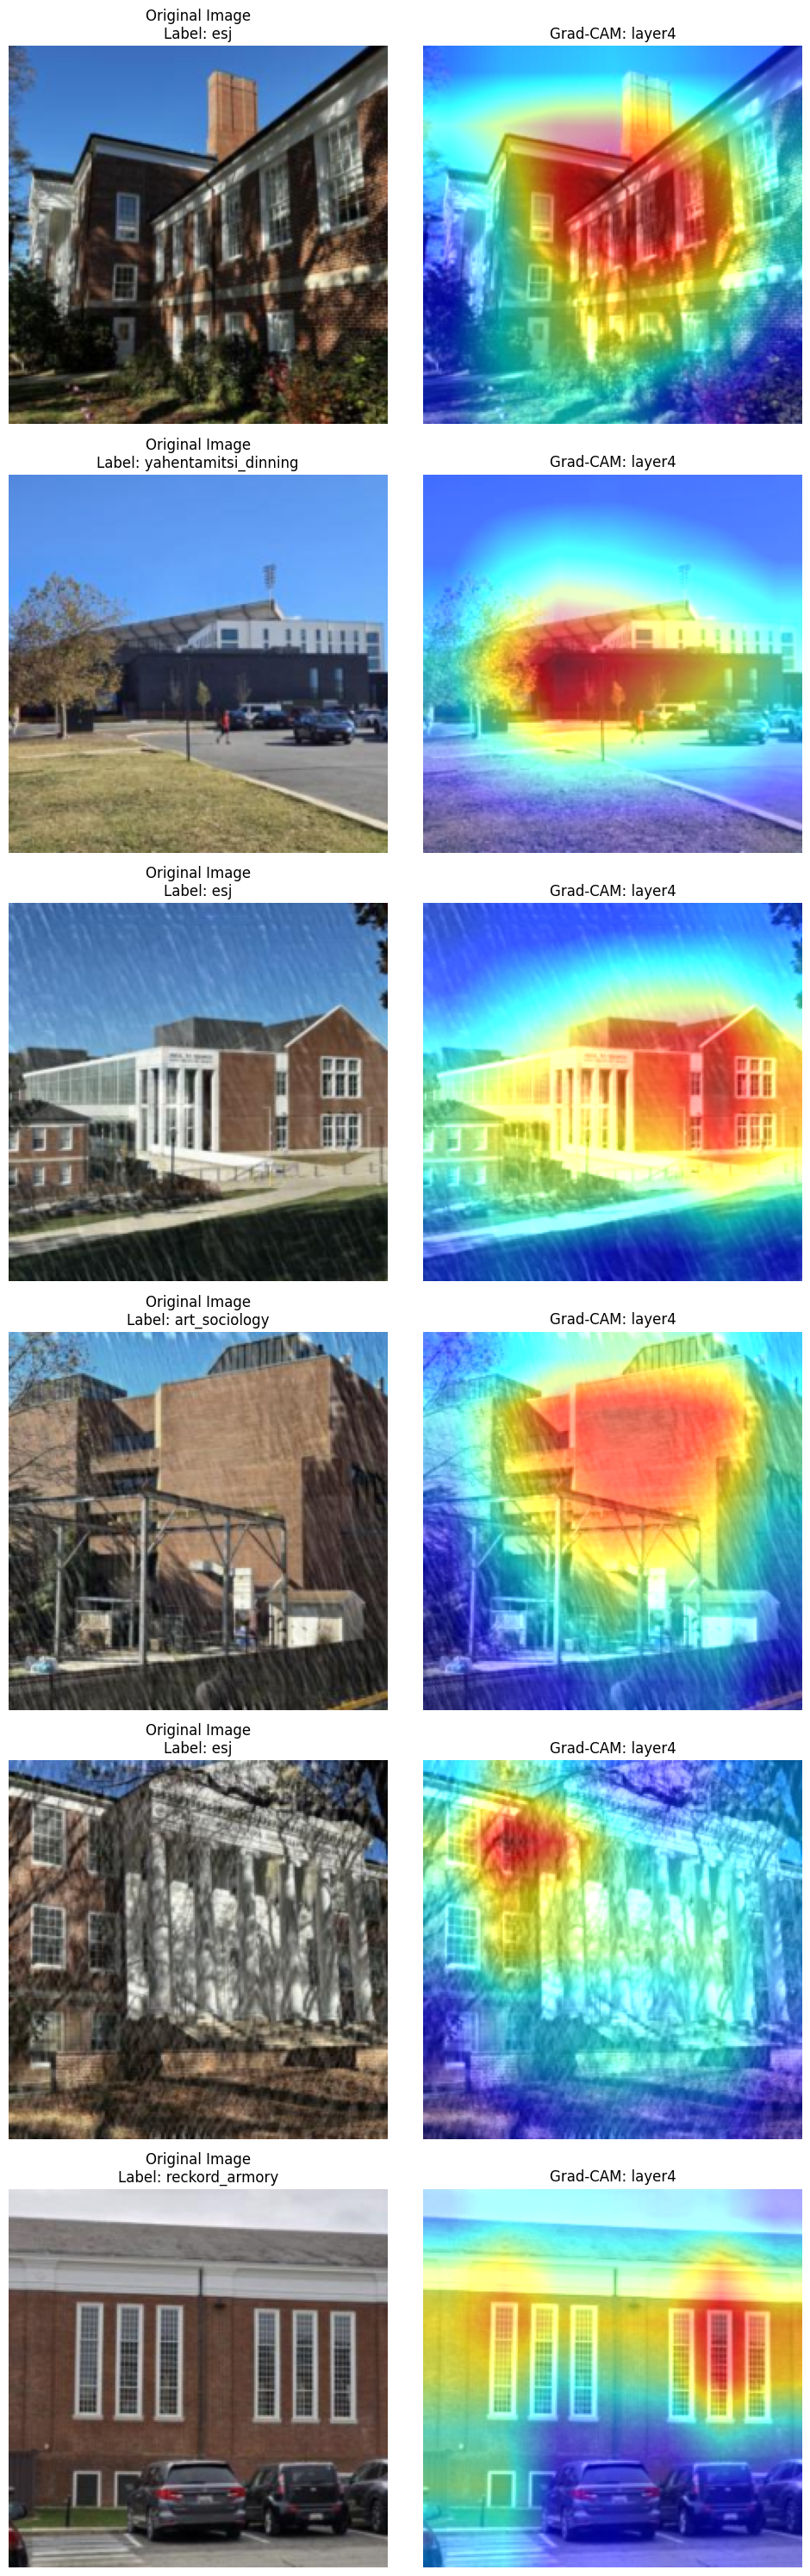
\includegraphics[width=\linewidth]{mean_teach_gradcam_plusplus.png}
        \caption{Grad-CAM++ visualization on MeanTeach}
        \label{fig:gradcam4}
    \end{subfigure}

    \caption{Comparison of Grad-CAM and Grad-CAM++ visualizations on MeanTeach}
    \label{fig:gradcam_comparison2}
\end{figure}

\medskip


\small

\bibliographystyle{abbrv}
\bibliography{sources}

% https://www.getbibtex.com

\end{document}